\documentclass[11pt]{cmspaperpdf}

\usepackage{amsmath}
\usepackage{epsfig}
\usepackage{subfigure}
\usepackage{graphicx}
\usepackage{multirow}

\newcommand{\pt}{\ensuremath{p_{\textrm{T}}}}
\newcommand{\et}{\ensuremath{E_{\textrm{T}}}}
\newcommand{\met}{\ensuremath{E_{\textrm{T}}^{\textrm{miss}}}}
\newcommand{\theht}{\ensuremath{H_{\textrm{T}}}}
\newcommand{\mht}{\ensuremath{H_{\textrm{T}}^{\textrm{miss}}}}

\begin{document}
\begin{titlepage}

\analysisnote{2015/XXX}

\date{\today}

%\newcommand{\mht}{H_{\rm T}^{\rm miss}}
%\newcommand{\mPt}{P_{\rm T}^{\rm miss}}
%\newcommand{\htt}{H_{\rm T}}
%

\title{Level-1 Jet Trigger Prefiring studies}

% >> Authors
\begin{Authlist}
 Georgia Karapostoli$^1$, Alex Tapper$^1$
\Instfoot{ic}{$^1$Imperial College London, UK.}
\end{Authlist}


\abstract{

}

\end{titlepage}
\tableofcontents

%%%%%%%%%%%%%%%
\newpage
\section{Introduction}

In this Note we study the possibility of Level-1 jet triggers prefiring, and particularly at high energies. Prefiring effects have not been a problem during 2010-2012 of the LHC running, as events firing at the wrong bunch-crossing were vetoed.

After LS1, however, the LHC will shift to operation with every 25~ns bucket filled, and such techniques will no longer be applicable to suppress the impact of spurious signals. The impact of this change on the Level-1 trigger has been estimated by studying the performance using 2012 data in the regions where 24 upgrade PMTs were already installed in the CMS detector.

Fig.~\ref{fig:hcaltdr_plot} refers to the Forward Calorimeter and refers to the prefiring generated by the signals in the PMT windows. Which we know can be a problem, indeed. That plot was computed using minimum bias events, but we extend this study to investigate the effect from high pT events: on minbias events one does not expect much prefiring from particles reaching the PMTs (in case of HF), or from a fraction of the signal leaking in the early bunch from HBHE. 

In this Note we try to clarify if this is a potential issue for the upcoming LHC 25ns run2, and to study the effect in case it is.

\vspace{5mm}
\begin{figure}[h!]
\centering
\setlength\fboxsep{0pt}
\setlength\fboxrule{0.2pt}
\fbox{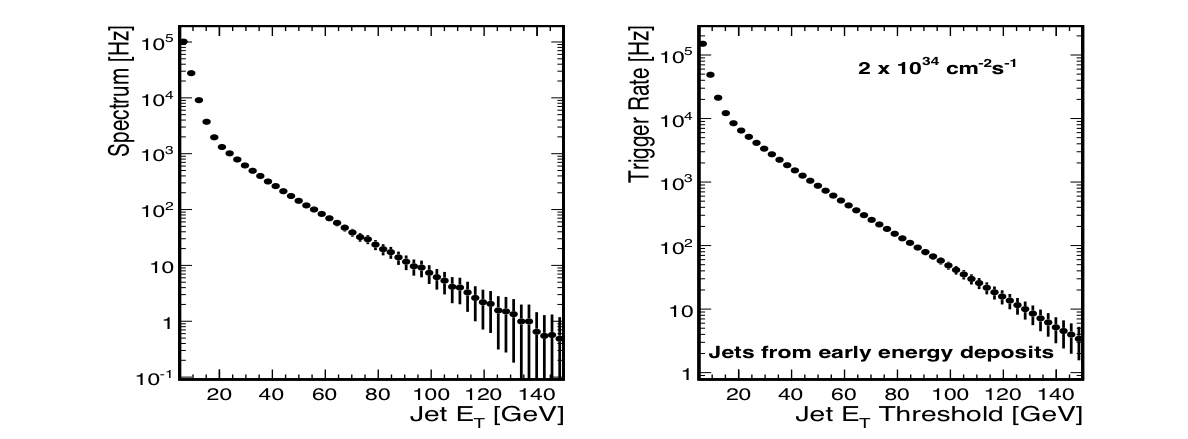
\includegraphics[scale=0.8]{plots/hcaltdr_plot.png}}
\caption{The spectrum of fake jets in HF induced by out-of-time jet candidates at Level-1, for an instantaneous luminosity of $2 \times 10^{34} \textrm{cm}^{-1} \textrm{s}^{-1}$. The plots are shown in the CMS TDR for the Phase I Upgrade of the Hadron Calorimeter under the section ``Background Rejection''~\cite{hcaltdr}.}
\label{fig:hcaltdr_plot}
\end{figure}
\vspace{5mm}

We perform studies similar to Fig.~\ref{fig:hcaltdr_plot}, but looking at higher energy events as well. We quantify the effect as a function of the pT of the Jets.

\newpage

\section{Framework and 2012 datasets}
\label{sec:tech}

As shown elsewhere~\cite{}, the performance of the L1 calorimeter trigger has been primarily evaluated with datasets collected using zero- or minimum-bias triggers. However these provide only adequate statistics for performance evaluation of calorimeter triggers with low energy thresholds. For higher energy thresholds, such event samples become insufficient to study trigger performance and events collected using a single muon trigger are used instead. This procedure has been shown to be unbiased for the triggers under study.

In this note, events from the ``SingleMu'' dataset were used to evaluate the performance at high energies:

\texttt{/SingleMu/Run2012D-PromptReco-v1/AOD}

The sample was further selected by filtering events based on isolated muon triggers (\texttt{HLT\_IsoMu}).

To cross-check the performance results with the ones presented in fig.~\ref{fig:hcaltdr_plot}, we also repeated the analysis using events from the minimum bias datasets:

\texttt{/MinimumBias/Run2012D-PromptReco-v1/AOD}

where events were further selected based on zero bias triggers (\texttt{HLT\_ZeroBias}).

In both cases, the analysis only used events certified with the Golden JSON file:

\texttt{Cert\_190456-208686\_8TeV\_PromptReco\_Collisions12\_JSON.txt}.

The events from the 2012 datasets above were analyzed within the official L1Ntuple framework~\cite{l1ntpl}. L1Ntuples were privately produced and further analyzed using a private Analyzer to evaluate the effect of pre-firing in the HCAL. The L1jet collections  were accessed using standard l1Extra candidates from all the available bunch-crossing (i.e. BX=-1, 0, 1). We split L1jets in ``central'' L1jet candidates using the OR of ``L1 cen jets'' and ``L1 tau jets'', and in ``forward'' L1jet candidates from the ``L1 FwdJet'' collection.

\section{Level-1 jet triggers}
\label{sec:l1jetalgo}

The Level-1 jet trigger uses the transverse energy sums computed in the calorimeter (both hadronic and electromagnetic) trigger regions. Each region consists of $4 \times 4 $  trigger tower windows, which each of them spans a region of $\Delta \eta \times \Delta \phi = 0.087 \times 0.087$ in pseudorapidity-azimuth. The jet trigger uses a $3 \times 3$ calorimeter region (112 trigger towers) sliding window technique which spans the full $(\eta, \phi)$ coverage
of the CMS calorimeter (Fig.~\ref{fig:l1jetalgo}). The central region \et ~is required to be higher than the eight neighbour region \et ~values,
and also be higher than a threshold, the latter to suppress noises. The L1 jets are characterised by the transverse energy \et, summed over the $3 \times 3$ calorimeter regions, which corresponds to $12 \times 12$ trigger towers in barrel and endcap or $3 \times 3$ larger HF towers in the HF. The $\phi$ size of the jet window is the same everywhere. The $\eta$ binning gets somewhat larger at high $\eta$  due to the size of the calorimeter and trigger tower segmentation. The jets are labelled by $(\eta, \phi)$ indexes of the central calorimeter region.

Jets with $|\eta|>3.0$ are classified as forward jets, whereas those with $|\eta|<3.0$ are classified as central or $\tau$, 
depending on the OR of the nine $\tau$-veto bits associated with the 9 regions in the $3 \times 3$ window. 
The four highest energy central and forward jets, and central $\tau$s in the calorimeter are selected. 
After jets are found, LUTs are used to apply a programmable $\eta-$dependent jet energy scale correction.

\begin{figure}[h!]
\centering
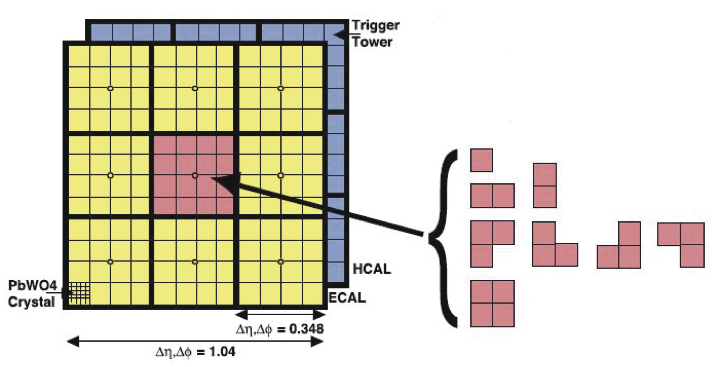
\includegraphics[scale=1.0]{plots/L1JetAlgorithm.png}
\caption{Illustration of the Level-1 jet finding algorithm.}
\label{fig:l1jetalgo}
\end{figure}
\vspace{5mm}


\section{Trigger pre-firing rates in HCAL}

A measure of the prefiring effect from L1jet triggers in the barrel-endcap (HBHE) and Forward (HF) regions of the hadronic calorimeter, is evaluated by calculating the relative rate of Jet triggers coming from early energy deposits in the HCAL, ie. L1jet candidates from BX=-1, with respect to the number of Jet triggers firing at the central BX(=0).

In the next two subsections, we evaluate the relative rate of L1jets prefiring in the HCAL as a function of the L1jet threshold, for the HBHE and HF regions separately.

\subsection{Prefiring rates in HCAL HB/HE}
\label{sec:rates_hbhe}

The pre-firing rate of L1jets in the HBHE region is estimated as a function of the L1jet \pt~threshold. Only the leading L1jet candidate (``cen jet'' or ``tau jet'') from each BX=-1,0 is used, as this is equivalent with a L1A from L1jet trigger firing. We plot the L1jet \pt~spectrum for Jets firing at the central BX(=0) and jets from early energy deposits appearing in BX=-1, for minimum bias events (see fig.~\ref{fig:l1jetpt_minb}) and single muon events (see fig.~\ref{fig:l1jetpt_smu}). We note that the peak at the $\pt=250$~GeV bin of the distributions corresponds to L1jet candidates with saturated \et. 

To calculate the relative rate of events prefiring in the HBHE region, we first integrate the distributions over the jet \pt~ spectrum, and extract a rate of events firing at BX=0 (black distributions) and a rate of events with L1jets prefiring at BX=-1 (red distributions). This is shown as a function of the L1jet \pt~threshold in both the minumum bias (fig.~\ref{fig:hbherate_minb}) and single muon (fig.~\ref{fig:hbherate_smu}) events. The rate is shown in arbitrary units. The ratio of the two distributions, namely the ratio between BX=-1 and BX=0 rates, gives a measure of the relative rate of prefiring.

%Noise: look at events with BX=0 L1jet of saturated ET --> single Event analysis

\begin{2figures}{h!}
\centering
\resizebox{1.\linewidth}{0.45\height}{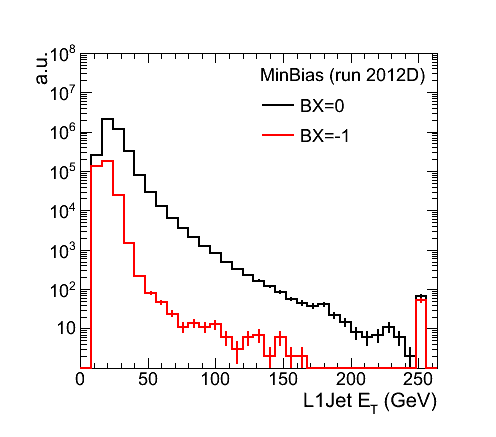
\includegraphics{plots/ptSpectrum_cenJets_MinBias_runD.png}} &
\resizebox{1.\linewidth}{0.45\height}{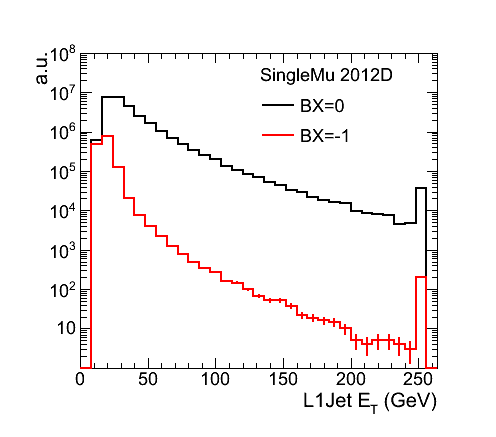
\includegraphics{plots/ptSpectrum_cenJets_SingleMu_runD.png}} \\
\caption{Level-1 Jet spectrum for central (black) and out-of-time (red) candidates in ``zerobias'' events with the 2012 runD dataset.}\label{fig:l1jetpt_minb}  &
\caption{Level-1 Jet spectrum for central (black) and out-of-time (red) candidates in ``single muon'' events with the 2012 runD dataset.}\label{fig:l1jetpt_smu}
\end{2figures}
\begin{2figures}{h!}
\centering
\resizebox{1.\linewidth}{0.45\height}{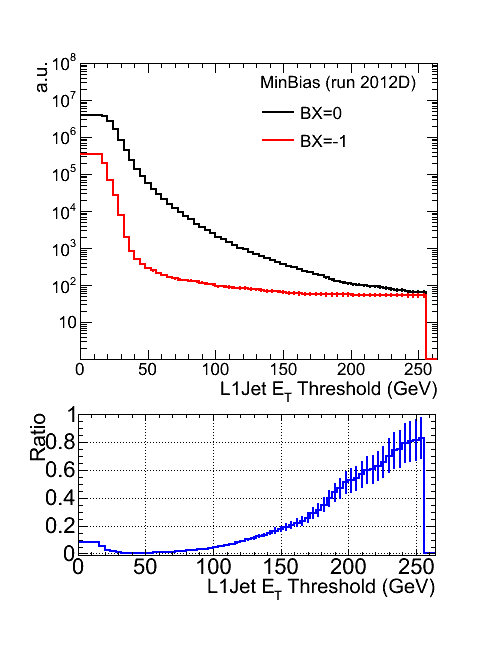
\includegraphics{plots/Rate_cenJets_MinBias_runD.png}} &
\resizebox{1.\linewidth}{0.45\height}{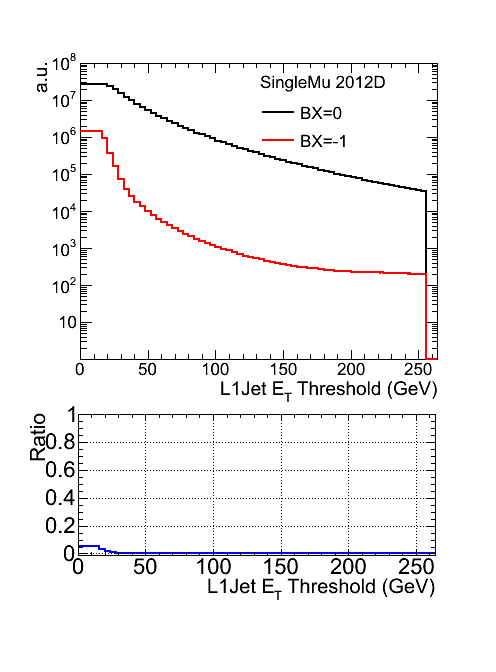
\includegraphics{plots/Rate_cenJets_SingleMu_runD.png}} \\
\caption{Level-1 Jet rate for central (black) and out-of-time (red) candidates in ``zerobias'' events with the 2012 runD dataset.}\label{fig:hbherate_minb} &
\caption{Level-1 Jet rate for central (black) and out-of-time (red) candidates in ``single muon'' events with the 2012 runD dataset.}\label{fig:hbherate_smu}
\end{2figures}

We notice at this point is that relative rates of early triggers show strikingly different between minimum bias and single muon events. This can be explained by the plots in figures~\ref{fig:l1jetpt_minb} and ~\ref{fig:l1jetpt_smu}, where the peak in the overflow bin of the L1jet spectrum in mimimum bias events shows approximately of the same size between L1jets at BX=-1 and Jets at BX=0. This is opposed to the single muon events, where the relative amount of Jet triggers between BX=-1 and BX=0 stays constant beyond a certain L1jet threshold.

The unexpectedly large peak in the overflow bin for the out-of-time (early) L1jet candidates in minimum bias events has been shown to be likely to noise. 
%We know that this should give a striped pattern in the Trigger Primitives (TPs) or one could check the HLT/offline where there are filters for this noise. Of course we do not have information either TPs, HLT or offline for the early BX but can check the peak for the in time BX. Therefore, this effect seems to be irreducible. 
To establish this assumption, we next investigate only the events with L1jets of saturated \et. We plot the $\eta$ and $\phi$ distributions for out of time L1jets of saturated \et~(fig.~\ref{fig:early_eta_phi}) and for in time L1jets of saturated \et~(fig.~\ref{fig:central_eta_phi}). As can be seen, out of time L1jets of saturated \et~ come predominantly from suspicious spikes in $\eta/\phi$, which is an observation consistent with noise. This effect seems to be irreducible at L1.
%Indeed, as we expected the distributions for out of time L1jets show spikes in $\eta$/$\phi$, as opposed to the distributions coming from genuine Jets at L1.

% Early L1jets with saturated Et in MinBias events
\begin{figure}
\centering
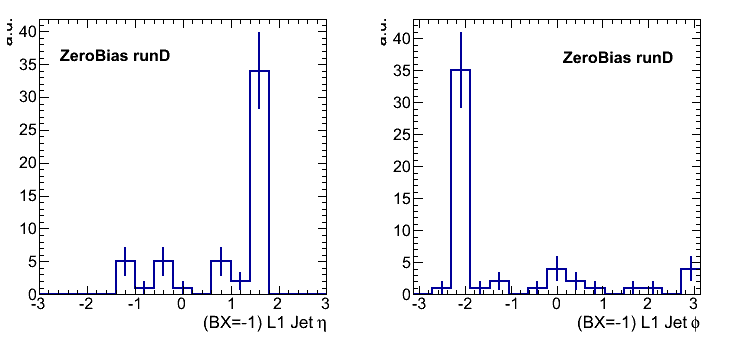
\includegraphics[scale=0.5]{plots/early_l1Jet_withSaturatedEt_eta_phi_ZeroBias_runD.png}
\caption{L1 Jet $\eta$ (left) and $\phi$ (right) distributions for candidates with saturated $E_{T}$ at the early BX=-1 (out of time L1jets) in minimum bias events with the 2012 runD datasets. }
\label{fig:early_eta_phi} 
\end{figure}
\begin{figure}
\centering
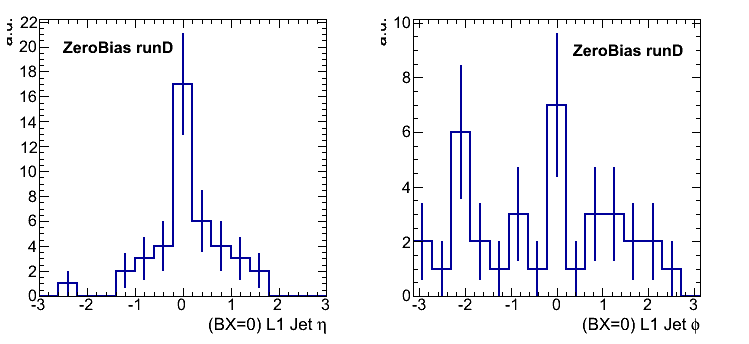
\includegraphics[scale=0.5]{plots/central_l1Jet_withSaturatedEt_eta_phi_ZeroBias_runD.png}
\caption{L1 Jet $\eta$ (left) and $\phi$ (right) for candidates with saturated $E_{T}$ at the central BX=0 (in time L1jets) in minimum bias events with the 2012 runD datasets.} 
\label{fig:central_eta_phi} 
\end{figure}

\newpage
\subsection{Prefiring rates in the Forward Calorimeter}
\label{sec:rates_hf}

A pre-firing rate is also evaluated for L1jets in the Forward Calorimeter. As in the previous subsection, we first show the L1jet \pt~spectrum of jets at BX=0 (in black) and BX=-1 (in red), both for minimum bias events (see fig.~\ref{fig:fwdjetpt_minb}) and single muon events (see fig.~\ref{fig:fwdjetpt_smu}). One can notice in this case, that the effect from the overflow bin in the distributions (jets with saturated \pt), gives rise and the plateau behavior in the relative rate of prefiring in a similar way between minimumbias and single muon events (figures~\ref{fig:fwdrate_minb} and~\ref{fig:fwdrate_smu}).

\begin{2figures}{h!}
\centering
\resizebox{1.\linewidth}{0.45\height}{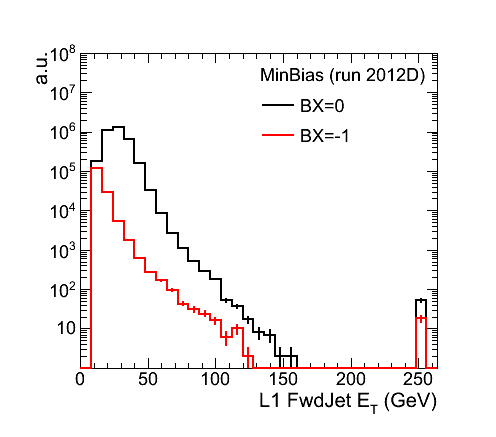
\includegraphics{plots/ptSpectrum_FwdJets_MinBias_runD.png}} &
\resizebox{1.\linewidth}{0.45\height}{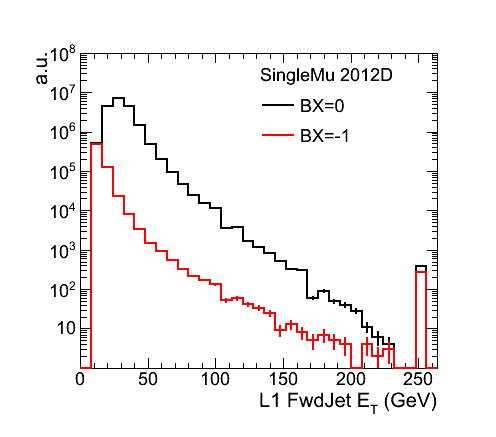
\includegraphics{plots/ptSpectrum_FwdJets_SingleMu_runD.png}} \\
\caption{Level-1 Jet spectrum in the Forward Calorimeter, for central (black) and out-of-time (red) candidates in ``zerobias'' events with the 2012 runD dataset.}\label{fig:fwdjetpt_minb} &
\caption{Level-1 Jet spectrum in the Forward Calorimeter, for central (black) and out-of-time (red) candidates in ``single muon'' events with the 2012 runD dataset.}\label{fig:fwdjetpt_smu}
\end{2figures}
\begin{2figures}{h!}
\centering
\resizebox{1.\linewidth}{0.45\height}{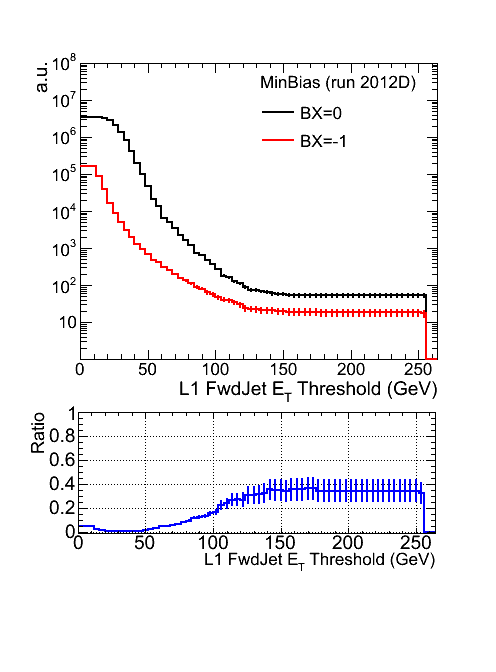
\includegraphics{plots/Rate_FwdJets_MinBias_runD.png}} &
\resizebox{1.\linewidth}{0.45\height}{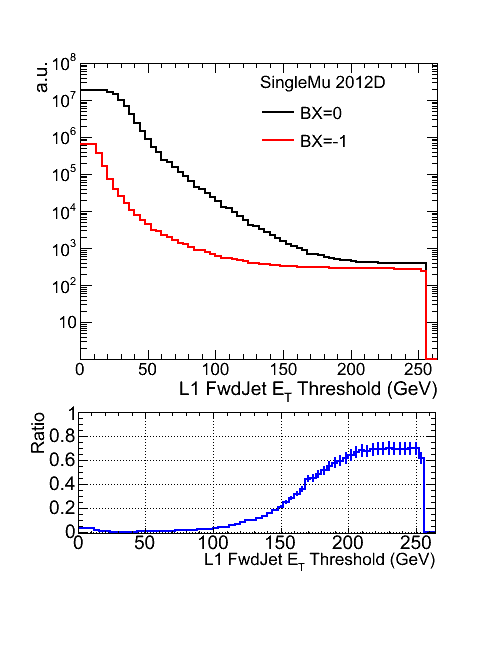
\includegraphics{plots/Rate_FwdJets_SingleMu_runD.png}} \\
\caption{Level-1 Jet rate in the Forward Calorimeter, for central (black) and out-of-time (red) candidates in ``zerobias'' events with the 2012 runD dataset.}\label{fig:fwdrate_minb} &
\caption{Level-1 Jet rate in the Forward Calorimeter, for central (black) and out-of-time (red) candidates in ``single muon'' events with the 2012 runD dataset.}\label{fig:fwdrate_smu}
\end{2figures}

\section{Impact of Upgraded Forward Calorimeter}

 In HF it was suggested that we look at the difference between the old and new PMTs in the 2012 data (as in the HCAL TDR). From private communication with HCAL experts, we were able to get the location of the upgraded PMTs that were already installed during the 2012 data taking period. A full list of ($i\eta,i\phi$) regions for the new PMTs is shown in fig.~\ref{fig:newpmts}, basically corresponding to $i \phi=43$~HF-. The same figure shows the new PMTs location in a L1jet ($i\eta,i\phi$) map.
%We have asked where the new PMTs are in the HF but we don't know the answer yet (it has been forgotten since the HCAL TDR and needs to be re-determined). 

With this information, we were able to get a low statistics test of what to expect in 2015 running. The expected reduction factors seemed to be from factor of 2 to factor of 5 or more, as have been mentioned by HCAL experts.
In our case, we made an attempt to extend the expected performance with the upgraded HF, at higher trigger energies. For this, we used the single muon dataset and compared the pre-firing rate in the region of the new PMTs ( $i \phi=43$~HF-) versus the rate in the region of other PMTs (e.g. here used  $i \phi=39$~HF-). This is shown separately for the two cases in figures~\ref{fig:oldpmts} and~\ref{fig:newpmts}. 

A direct comparison is given by the ratio of the two pre-firing rates as shown in fig.~\ref{fig:imp}, indicating a lower limit on the expected improvement with a reduction factor of $3-4$ for jet \pt~thresholds greater than 100~GeV\footnote{The L1jets are much bigger than the area of the new PMTs, so the upgraded performance shown in fig.~\ref{fig:newpmts} comes from  a mixture of the old and new PMTs.}.

\begin{figure}
\centering
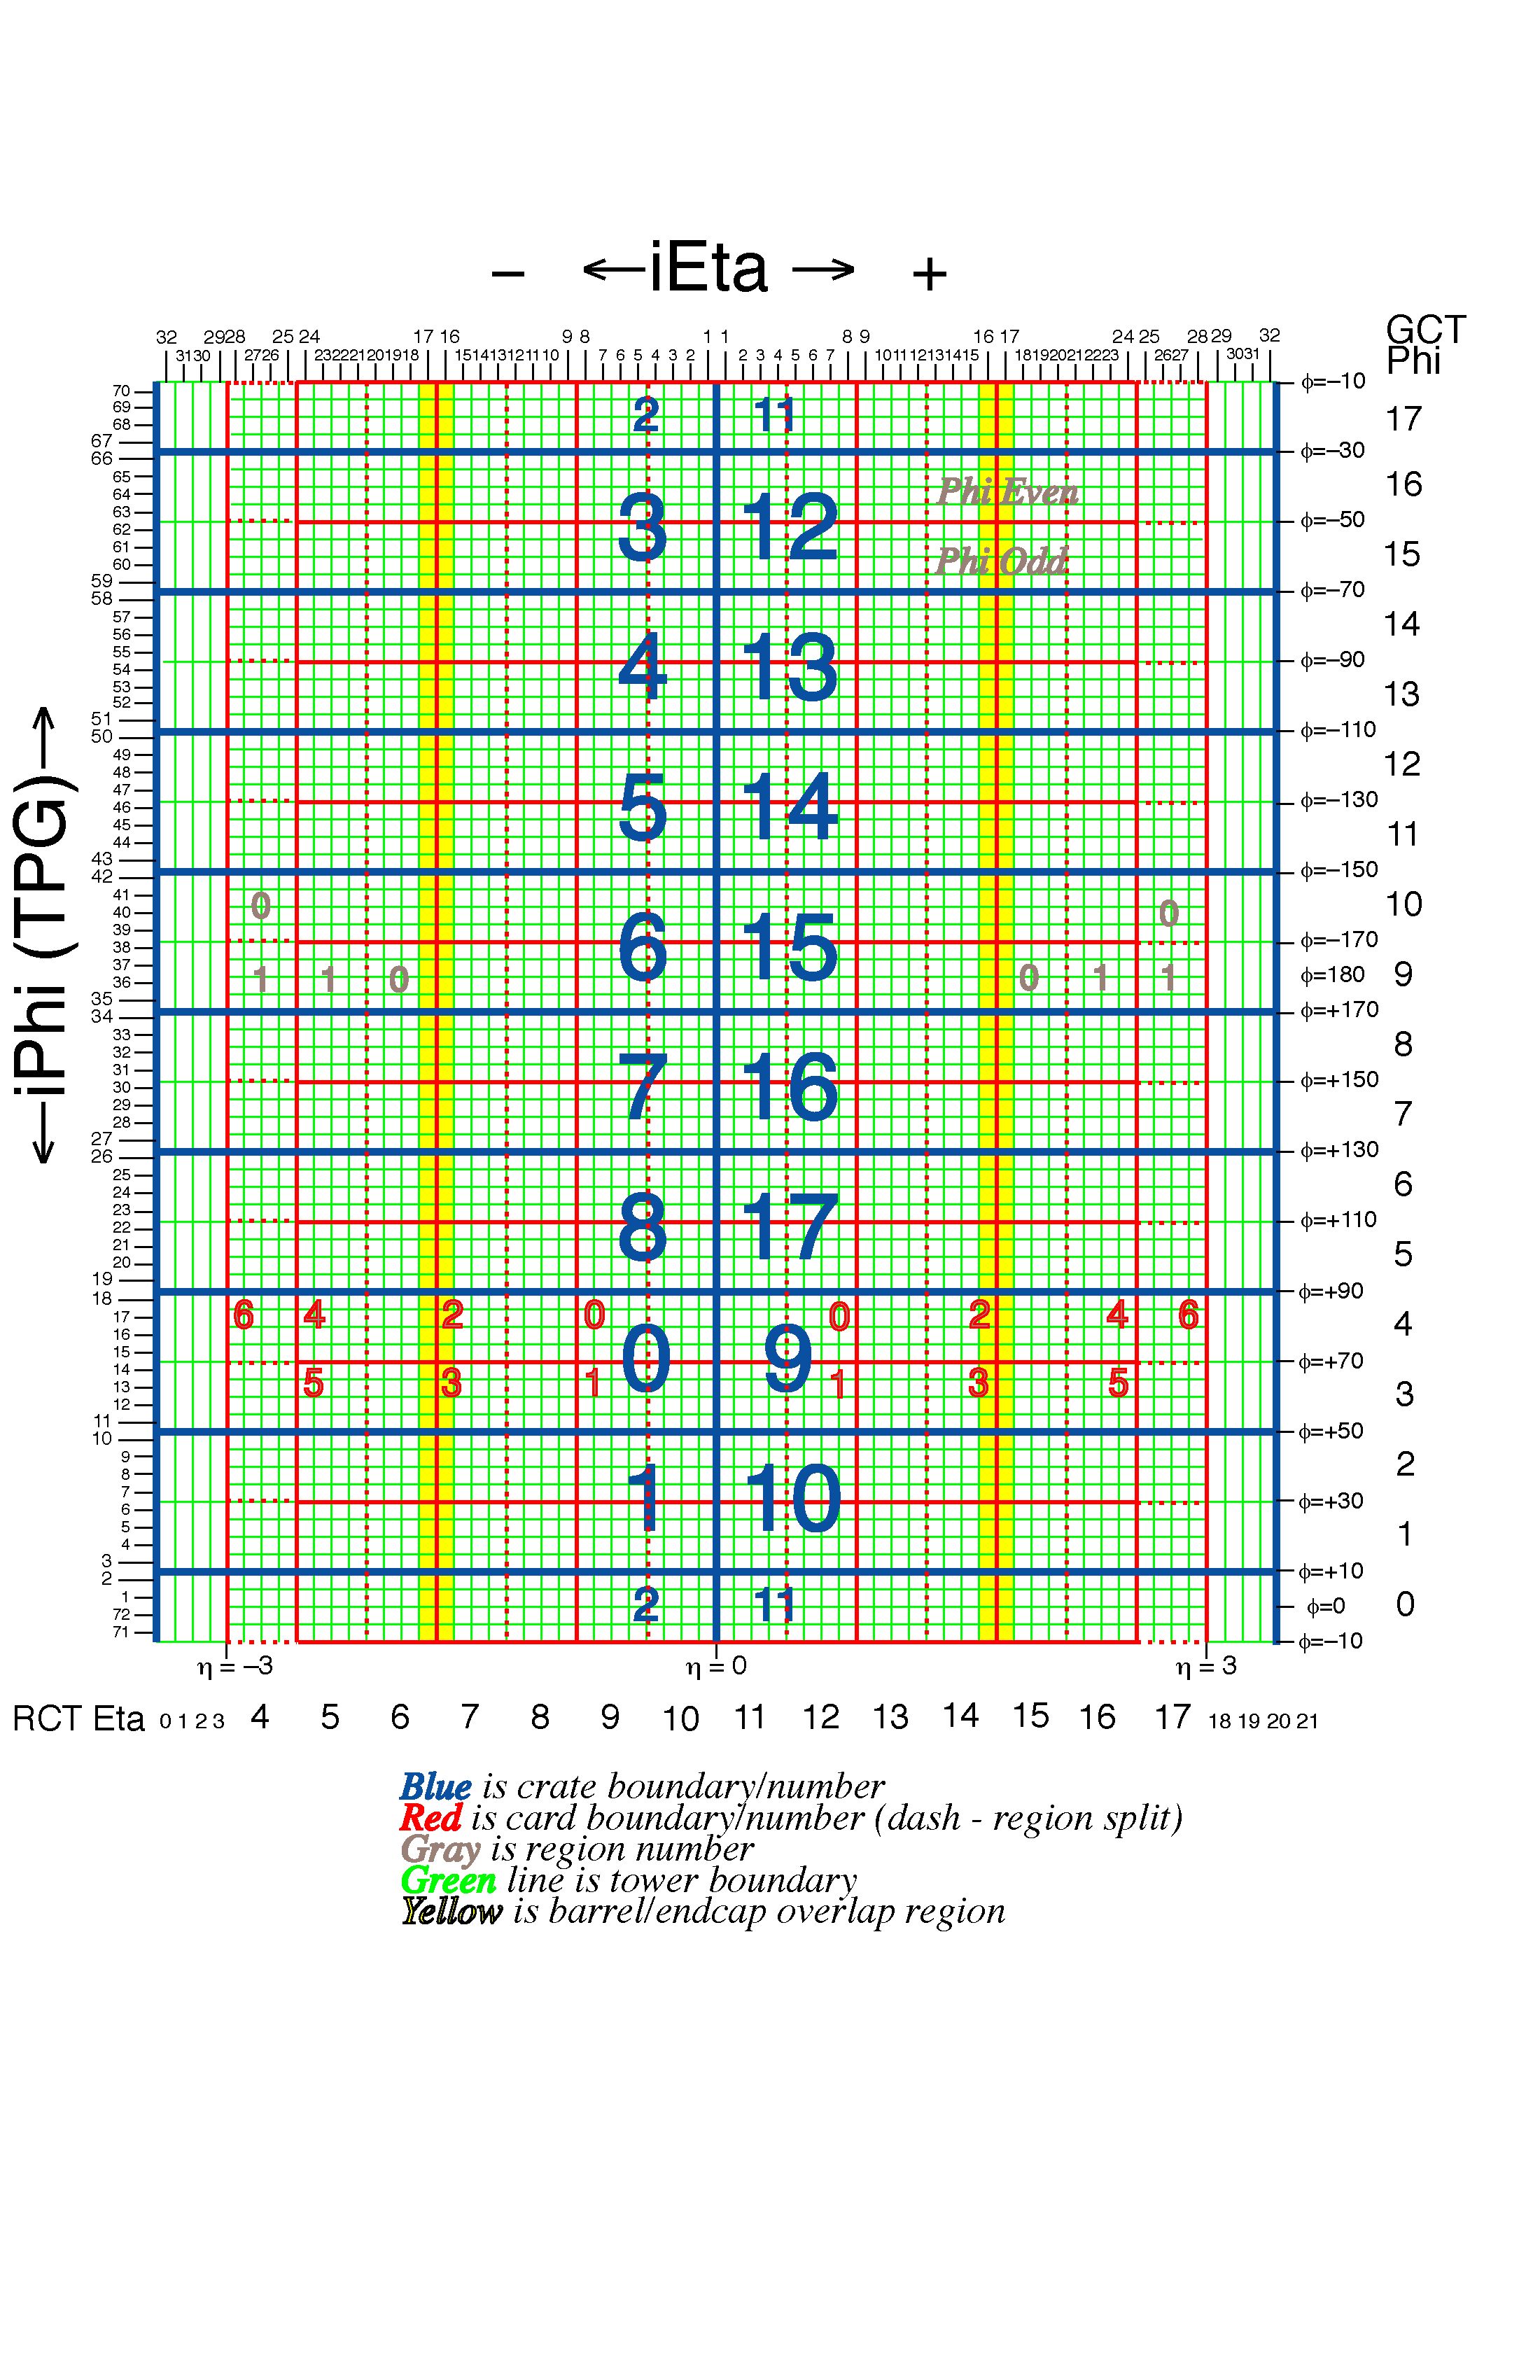
\includegraphics[scale=0.23]{plots/towers_ieta_iphi_2009.png}
\caption{Regional calorimeter trigger map in trigger tower space.} 
\end{figure}
\vspace{5mm}

\begin{figure}
\centering
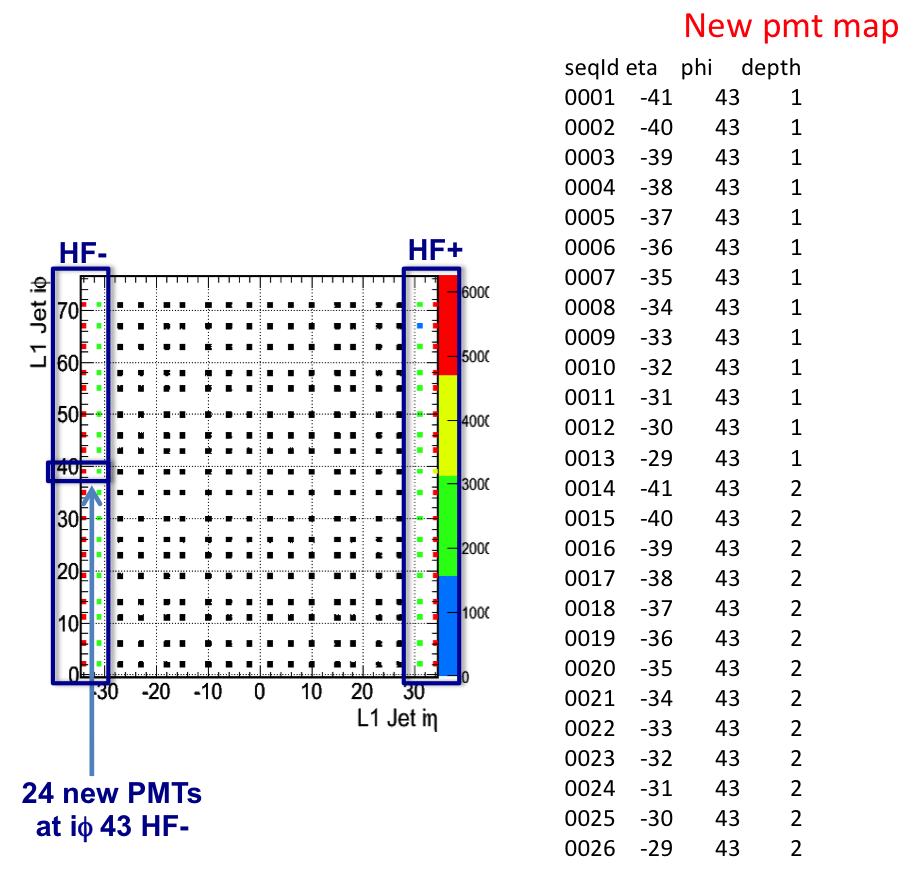
\includegraphics[scale=0.7]{plots/upgradedPMTs_regions_in2012.png}
%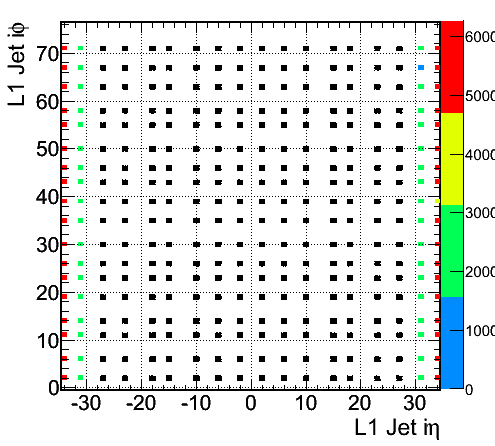
\includegraphics[scale=0.5]{plots/l1Jet_ieta_iphi_BX0_fullmap.png}
\caption{L1 jet ($\eta$,$\phi$) mapped to ($i \eta$, $i \phi$) tower detID. Black dots correspond to L1Jets falling into the HB/HE regions, whereas color dots correspond the L1jets in the Forward Calorimeter ($| i \eta| > 28$). The regions where the upgraded PMTs were installed during the 2012 data is shown superimposed at $i \phi=43$~HF-. }
\label{fig:newpmts} 
\end{figure}
 
\begin{2figures}{h!}
\centering
\resizebox{1.\linewidth}{0.45\height}{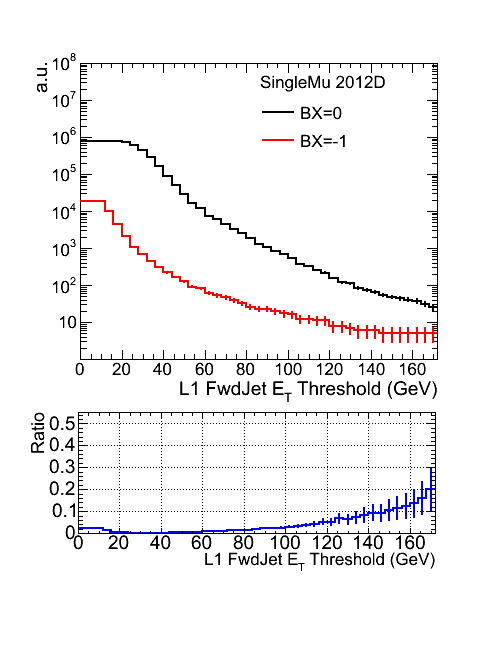
\includegraphics{plots/oldPMTs_Rate_FwdJets_SingleMu_runD.png}} &
\resizebox{1.\linewidth}{0.45\height}{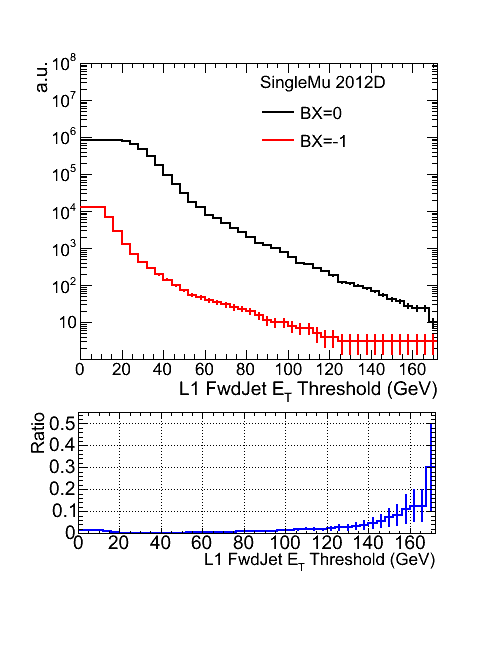
\includegraphics{plots/upgradedPMTs_Rate_FwdJets_SingleMu_runD.png}} \\
\caption{Level-1 Jet rate in the Forward Calorimeter, for central (black) and out-of-time (red) candidates in ``single muon'' events with the 2012 runD dataset. L1 jets fall into regions with $i \phi=39$ HF- (old PMTs region).}\label{fig:oldpmts} &
\caption{Level-1 Jet rate in the Forward Calorimeter, for central (black) and out-of-time (red) candidates in ``single muon'' events with the 2012 runD dataset. L1 jets fall into regions with $i \phi=43$ HF- (regions with upgraded PMTs).}\label{fig:newpmts}
\end{2figures}
\begin{figure}
\centering
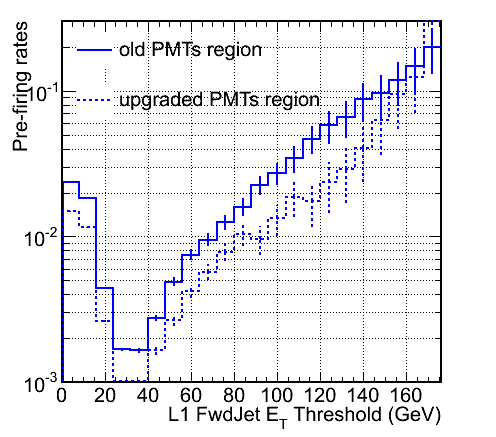
\includegraphics[scale=0.45]{plots/rates_comparison_old-vs-new-PMTs.png}
\caption{Prefiring rates comparison for L1jets falling into $i \phi=39$ HF- (old PMTs region) shown in solid blue, and $i \phi=43$ HF- (i.e. regions with upgraded PMTs) shown in dashed blue. }
\label{fig:imp} 
\end{figure}
 
%Upgraded PMTs analysis: iphi=43 L1 HFjets only. Need to know that 4x4 trigger towers=1 calorimeter region. h/phi of jet is in the centre of a calo region.

\newpage
\section{Performance with TSG physics skims}

We finally looked at the effect of pre-firing in some 2012D physics skims provided by the CMS Trigger Studies Group (TSG)~\cite{tsg}. The physics samples used for this analysis include events with W/Z decaying to leptons, $t \bar{t}$ events, $H \rightarrow WW$ as well as $H \rightarrow \tau\tau$ events. All events come from 2012D datasets selected based on some pre-defined trigger paths which enchance the signal events.

Figures~\ref{fig:p1_hbhe},~\ref{fig:p2_hbhe},~\ref{fig:p3_hbhe} and~\ref{fig:p4_hbhe} show the prefiring rates in HBHE regions, whereas figures~\ref{fig:p1_hf},~\ref{fig:p2_hf},~\ref{fig:p3_hf} and~\ref{fig:p4_hf} show the prefiring rates in HF. From the above we conclude that the pre-firing effect has been shown to be negligible for pure physics samples.

\begin{2figures}{h!}
\centering
\resizebox{1.\linewidth}{0.45\height}{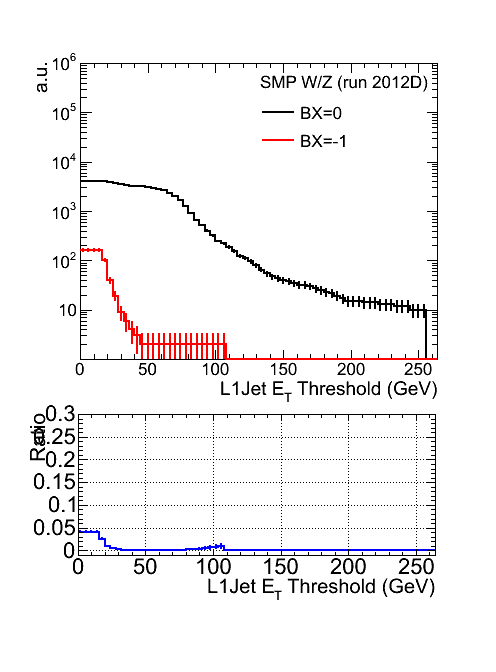
\includegraphics{plots/l1Jet_rate_HBHE_SMP_WZ_TSGskim.png}} &
\resizebox{1.\linewidth}{0.45\height}{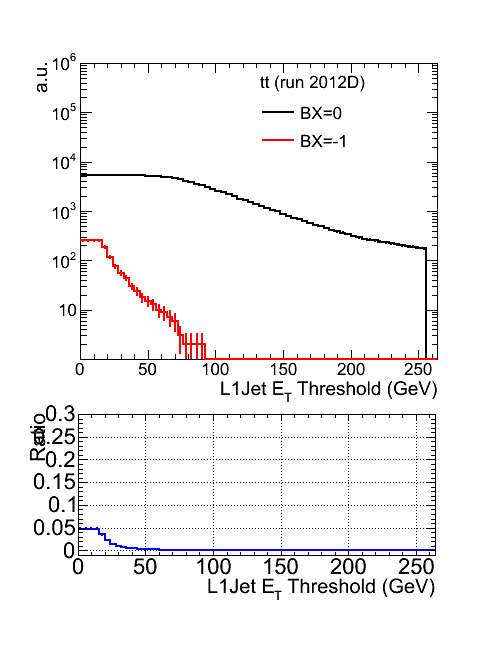
\includegraphics{plots/l1Jet_rate_HBHE_tt_TSGskim.png}} \\
\caption{Level-1 Jet rate for central (black) and out-of-time (red) candidates in $W/Z \rightarrow$ leptons events, for HBHE regions.}\label{fig:p1_hbhe} &
\caption{Level-1 Jet rate for central (black) and out-of-time (red) candidates in $t \bar{t}$ events, for HBHE regions.}\label{fig:p2_hbhe}
\end{2figures}
\begin{2figures}{h!}
\centering
\resizebox{1.\linewidth}{0.45\height}{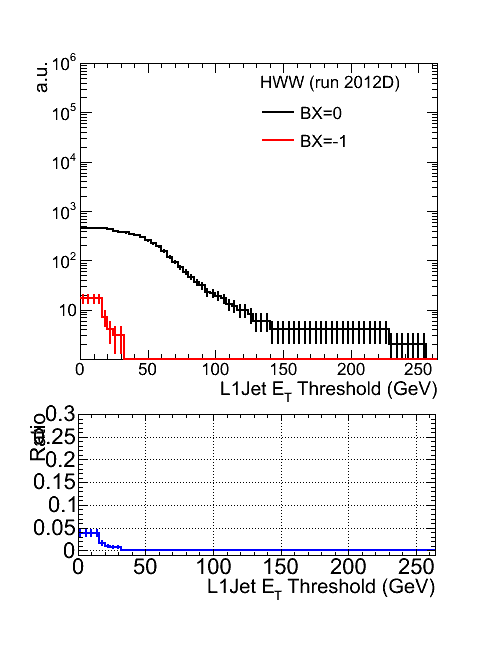
\includegraphics{plots/l1Jet_rate_HBHE_HWW_TSGskim.png}} &
\resizebox{1.\linewidth}{0.45\height}{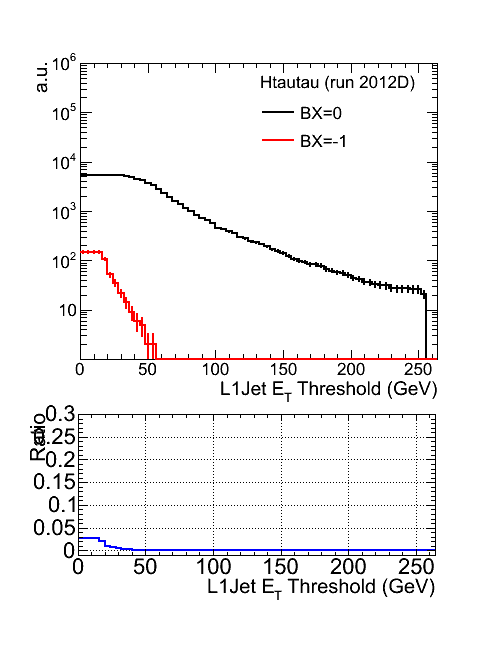
\includegraphics{plots/l1Jet_rate_HBHE_Htautau_TSGskim.png}} \\
\caption{Level-1 Jet rate for central (black) and out-of-time (red) candidates in $ H \rightarrow WW$ events, for HBHE regions.}\label{fig:p3_hbhe} &
\caption{Level-1 Jet rate for central (black) and out-of-time (red) candidates in $ H \rightarrow \tau \tau$ events, for HBHE regions.}\label{fig:p4_hbhe}
\end{2figures}

% TSG skims at HF
\begin{2figures}{h!}
\centering
\resizebox{1.\linewidth}{0.45\height}{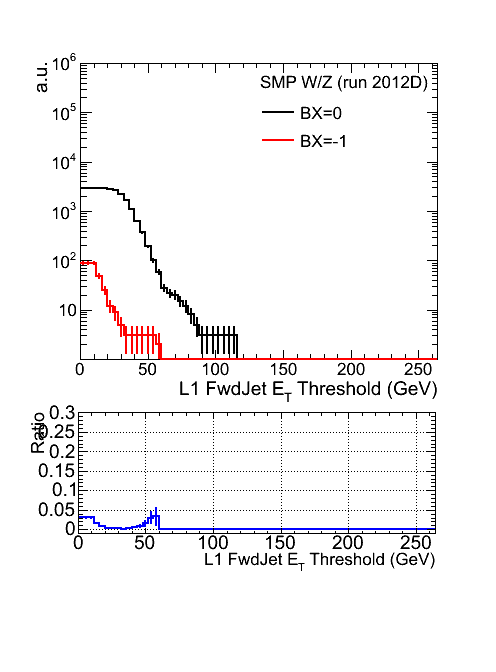
\includegraphics{plots/l1Jet_rate_HF_SMP_WZ_TSGskim.png}} &
\resizebox{1.\linewidth}{0.45\height}{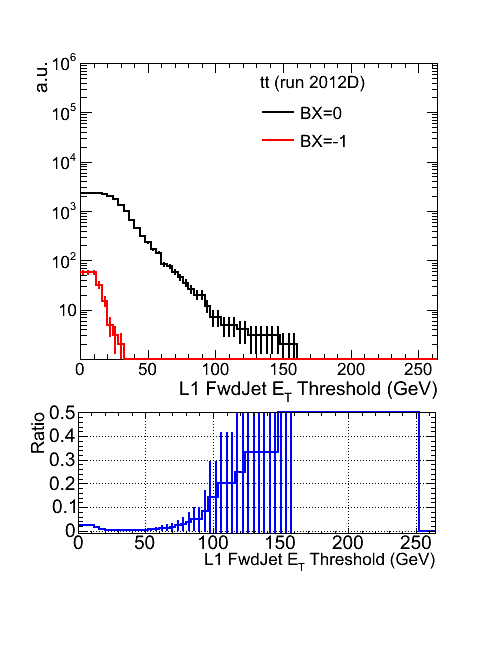
\includegraphics{plots/l1Jet_rate_HF_tt_TSGskim.png}} \\
\caption{Level-1 Jet rate for central (black) and out-of-time (red) candidates in $W/Z \rightarrow$ leptons events, in the HF region.}\label{fig:p1_hf} &
\caption{Level-1 Jet rate for central (black) and out-of-time (red) candidates in $t \bar{t}$ events, in the HF region.}\label{fig:p2_hf}
\end{2figures}
\begin{2figures}{h!}
\centering
\resizebox{1.\linewidth}{0.45\height}{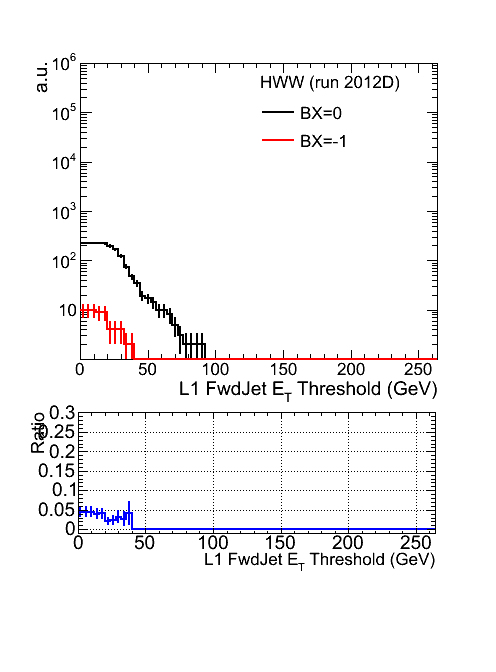
\includegraphics{plots/l1Jet_rate_HF_HWW_TSGskim.png}} &
\resizebox{1.\linewidth}{0.45\height}{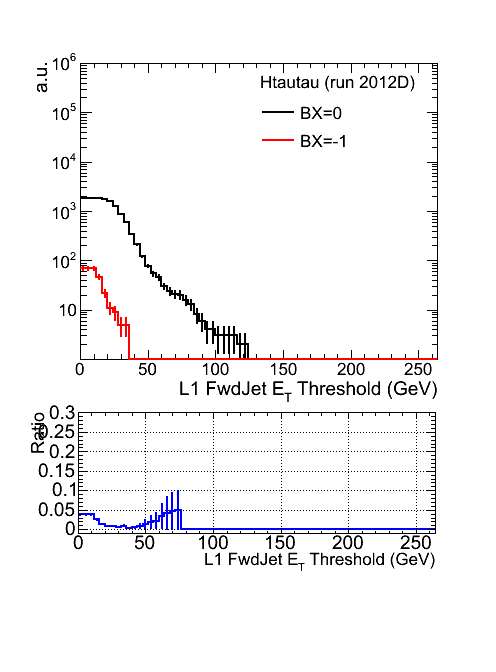
\includegraphics{plots/l1Jet_rate_HF_Htautau_TSGskim.png}} \\
\caption{Level-1 Jet rate for central (black) and out-of-time (red) candidates in $ H \rightarrow WW$ events, in the HF region.}\label{fig:p3_hf}  &
\caption{Level-1 Jet rate for central (black) and out-of-time (red) candidates in $ H \rightarrow \tau \tau$ events, in the HF region.}\label{fig:p4_hf} 
\end{2figures}

\section{Summary}

We think we've shown that the pre-firing from noise in HB/HE is not really a worry and quantified the pre-firing in HF as it was in 2012. The analysis of the replaced PMTs in HF is inconclusive since their effect is diluted by the large number of PMTs summed in a jet. 


\newpage
%% **DO NOT REMOVE BIBLIOGRAPHY**
\bibliography{auto_generated}   % will be created by the tdr script.

\begin{thebibliography}{99}

\bibitem{hcaltdr} ``CMS Technical Design Report for the Phase I Upgrade of the Hadron Calimeter'', CMS-TDR-010, CERN-LHCC-2012-015.
\bibitem{l1ntpl} https://twiki.cern.ch/twiki/bin/viewauth/CMS/L1TriggerDPGNtupleProduction .
\bibitem{tsg} https://twiki.cern.ch/twiki/bin/viewauth/CMS/HLTDataSkimsForValidation .

\end{thebibliography}

%% examples of appendices. **DO NOT PUT \end{document} at the end
\clearpage
\appendix

\end{document}


